\chapter{Corriente alterna}
\section{Fasores y corrientes alternas}
Para suministrar una corriente alterna a un circuito se requiere una fuente de fem o voltaje alternos.

Se aplica el término \textbf{fuente de ca} a cualquier dispositivo que suministre un voltaje (diferencia de potencial) $v$ o corriente $i$ que varía en forma sinusoidal.


Un voltaje sinusoidal queda descrito por una función como
\begin{equation}\label{31.1	}
v=V\cos\omega t 
\end{equation}
donde $v$ es la diferencia de potencial \textit{instantánea}; $V$ es la diferencia de potencial máxima, y se llama \textbf{amplitud del voltaje}; y $\omega$ es la \textit{frecuencia angular}, igual a $2\pi$ la frecuencia $f$. Una corriente sinusoidal se describe como

\begin{equation}\label{31.2}
\boxed{i=I\cos\omega t}
\end{equation}

donde $i$ es la corriente instantánea, e $I$ es la corriente máxima o \textbf{amplitud de corriente}.

\subsection{Diagramas de fasores}
En estos diagramas el valor instantáneo de una cantidad que varía sinusoidalmente con respecto al tiempo se representa mediante la proyección sobre un eje horizontal de un vector con longitud igual a la amplitud de la cantidad. El vector gira en el sentido antihorario con rapidez angular constante $\omega$. Estos vectores giratorios reciben el nombre de \textbf{fasores}, y los diagramas que los contienen se llaman \textbf{diagramas de fasores}.

\begin{figure}[h]
\centering
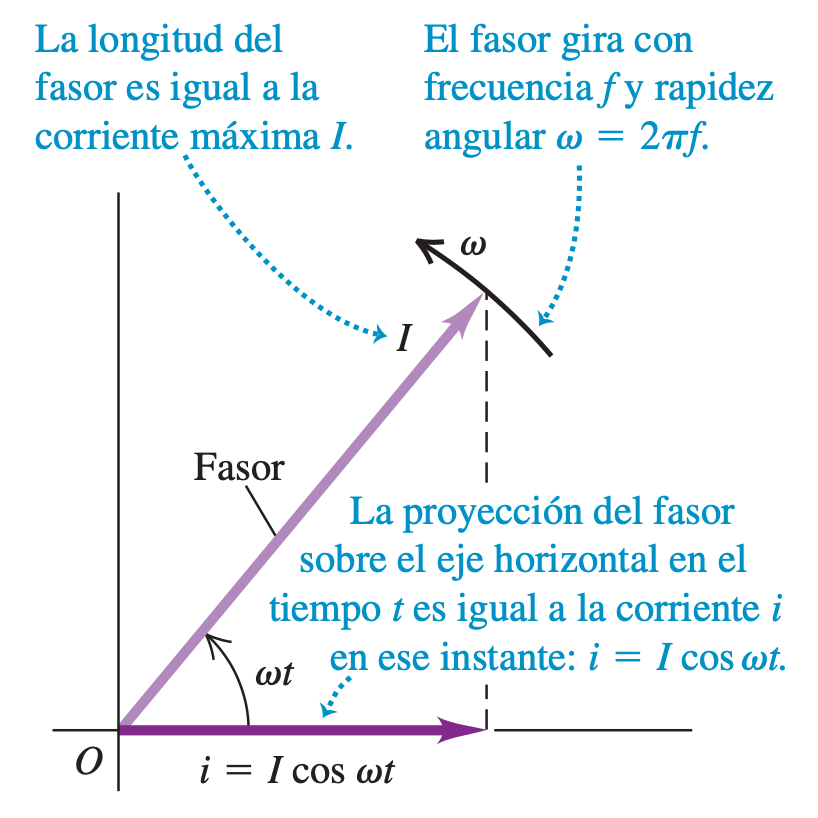
\includegraphics[scale=0.4]{fig/fasor1}
\caption{Diagrama de fasores}
\label{fig:fasor1}
\end{figure}










